\documentclass{article}
\usepackage{amsmath}
\usepackage{titlesec}
\usepackage{graphicx}
\usepackage[margin=1in]{geometry}
\usepackage{hyperref}
\usepackage{amssymb}
\usepackage{bm}


% Title, date, and author
\title{Exercise 4}
\author{Your Name, Collaborator's Name}
\date{\today}

\titleformat{\section}
  {\normalfont\normalsize\bfseries} % Format: font style, size, and weight
  {\thesection}{1em} % Label format and spacing
  {}
  \renewcommand{\thesubsection}{\thesection.\alph{subsection}}

\titleformat{\subsection}
  {\normalfont\small\bfseries} % Format: font style, size, and weight
  {\thesubsection}{1em} % Label format and spacing
  {}
\titleformat{\subsubsection}
  {\normalfont\small\bfseries} % Format: font style, size, and weight
  {\thesubsubsection}{1em} % Label format and spacing
  {}

\begin{document}
\begin{titlepage}
    \centering
    \vspace*{1in}
    
    {\Huge\bfseries Exercise 4\par}
    \vspace{1.5cm}
    {\Large \today\par}
    \vspace{1.5cm}
    {\Large\itshape Antonio Pampalone 23586519 \\ Giuseppe Pisante 23610012\\ Martina Raffaelli 23616907 \par}
    
    \vfill
    
\includegraphics[width=0.3\textwidth]{FAU-Logo.png}\par\vspace{1cm} % Adjust the width as needed
   
\end{titlepage}

\newpage
\small
\section{Steady advaction-diffusion equation}
\subsection{Non-dimensional form of the equation and boundary conditions}
Starting from the one-dimensional advection-diffusion equation:
\begin{equation} \label{initialeq}
    \rho \left(\frac{\partial \Phi}{\partial t} + U \frac{\partial \Phi}{\partial x}\right) = \alpha \frac{\partial^2 \Phi}{\partial x \partial x} 
\end{equation}
we derive the non-dimensional form of the equation by introducing the following non-dimensional variables:
\[
    x^* = \frac{x}{L}, \quad t^* = \frac{t}{T}, \quad \Phi^* = \frac{\Phi }{\Phi_L}
\]
where $L$ is a characteristic length, $T = \tfrac{L}{U}$ is the characteristic advection time, and $\Phi_L$ is a characteristic value of the variable $\Phi$.

Then we perform the change of the variable for the deivatives:
\[
    \frac{\partial}{\partial x} = \frac{1}{L} \frac{\partial}{\partial x^*}, \quad \frac{\partial}{\partial t} = \frac{1}{T} \frac{\partial}{\partial t^*}, \quad \frac{\partial^2}{\partial x \partial x} = \frac{1}{L^2} \frac{\partial^2}{\partial x^{*2}}
\]

Now we substitute the relations above into the original equation:
\[
    \rho \left(\frac{\Phi_L}{T} \frac{\partial \Phi^*}{\partial t^*} + U \frac{\Phi_L}{L} \frac{\partial \Phi^*}{\partial x^*}\right) = \alpha \frac{\Phi_L}{L^2} \frac{\partial^2 \Phi^*}{\partial x^{*2}}
\]
This equation can be simplified by dividing by $\Phi_L$ (assuming the quantity is not zero) and observing that $T = \tfrac{L}{U}$:
\[
    \rho \left(\frac{U}{T} \frac{\partial \Phi^*}{\partial t^*} + \frac{U}{L} \frac{\partial \Phi^*}{\partial x^*}\right) = \alpha \frac{1}{L^2} \frac{\partial^2 \Phi^*}{\partial x^{*2}}
\]
now we multiply for $\frac{L}{\rho U}$ and we get the following eqaution:
\[
    \frac{\partial \Phi^*}{\partial t^*} +  \frac{\partial \Phi^*}{\partial x^*} = \frac{\alpha}{\rho U L} \frac{\partial^2 \Phi^*}{\partial x^{*2}}
\]
where we can substitute the Peclet number $Pe = \tfrac{U L}{\alpha}$ to obtain the non-dimensional form of the equation \eqref{initialeq}:
\begin{equation} \label{non-dim}
    \frac{\partial \Phi^*}{\partial t^*} +\frac{\partial \Phi^*}{\partial x^*} = \frac{1}{Pe} \frac{\partial^2 \Phi^*}{\partial x^{*2}} 
\end{equation}

Now we repeat the same procedure for the boundary condistions, starting from the dimensional ones:
\begin{equation} \label{bc}
    \Phi(0, t) = 0, \quad \Phi(L, t) = \Phi_L
\end{equation}
and performing the change of variable: $x = 0$ becomes $x^* = 0$ and $x = L$ becomes $x^* = 1$.
Thus, the non-dimensional boundary conditions are:
\begin{equation} \label{non-dim-bc}
    \Phi^*(0, t^*) = 0, \quad \Phi^*(1, t^*) = 1
\end{equation}

\subsection{Analytical solution of the steady non-dimensional equation}
The steady non-dimensional equation is obtained by setting the time derivative to zero in \eqref{non-dim}:
\begin{equation} \label{steady}
    Pe \frac{\partial \Phi^*}{\partial x^*} = \frac{\partial^2 \Phi^*}{\partial x^{*2}}
\end{equation}
which represents a second-order ordinary differential equation. The general solution of this equation is:
\[
    \Phi^*(x^*) = C_1 e^{\lambda_1 x^*} + C_2 e^{\lambda_2 x^*}
\]
where $\lambda_1$ and $\lambda_2$ are the roots of the characteristic equation, which can be found by substituting $\Phi^*(x^*) = e^{\lambda x^*}$ into the ODE, as follows:
\[
    \lambda^2 e^{\lambda x^*} = Pe \lambda e^{\lambda x^*} \quad \Rightarrow \quad \lambda^2 = Pe \lambda \quad \Rightarrow \quad \lambda = 0, \lambda = Pe
\]

Then we have to find the constants $C_1$ and $C_2$ by imposing the boundary conditions \eqref{non-dim-bc}:
\[
    \Phi^*(0) = C_1 + C_2 = 0, \quad \Phi^*(1) = C_1 e^{0} + C_2 e^{Pe} = 1
\]
from which we get:
\[
    C_1 = - C_2, \quad C_2 = \frac{1}{1 - e^{Pe}}
\]
and the final solution is:
\begin{equation} \label{analyticalsolution}
    \Phi^*(x^*) = \frac{e^{x^* Pe} - 1}{e^{Pe} - 1}
\end{equation}

\subsection{Discretization of the steady non-dimensional equation}
\subsubsection*{Diffusion term discretization}
We discretize the diffusion term with the central finite differencing scheme:
\begin{equation} \label{diffusion}
    \frac{1}{Pe} \frac{\partial^2 \Phi^*}{\partial x^{*2}} \approx \frac{1}{Pe} \frac{\Phi^*_{i+1} - 2 \Phi^*_i + \Phi^*_{i-1}}{\Delta x^{*2}}
\end{equation}

\subsubsection*{Advection term discretization}
For the advection term we use different approaches:
\begin{itemize}
\item Second-order central differencing: 
\begin{equation} \label{advection}
    \frac{\partial \Phi^*}{\partial x^*} \approx \frac{\Phi^*_{i+1} - \Phi^*_{i-1}}{2 \Delta x^*}
\end{equation}

\item First-order upwind differencing:
\begin{equation} \label{upwind}
    \frac{\partial \Phi^*}{\partial x^*} \approx \frac{\Phi^*_{i} - \Phi^*_{i-1}}{\Delta x^*}
\end{equation}
\item Second-order upwind differencing:
\begin{equation} \label{upwind2}
    \frac{\partial \Phi^*}{\partial x^*} \approx \frac{3 \Phi^*_{i} - 4 \Phi^*_{i-1} + \Phi^*_{i-2}}{2 \Delta x^*}
\end{equation}
\end{itemize}

\subsection{Matrix form of the discretized equation}
To obtain the matrix formulations we have to match the discretizations of the the advection term with the one for the diffusion term.
\subsubsection*{Second-order central differencing for the advection term}
\begin{equation}
    \frac{1}{Pe} \frac{\Phi^*_{i+1} - 2 \Phi^*_i + \Phi^*_{i-1}}{\Delta x^{*2}} = \frac{\Phi^*_{i+1} - \Phi^*_{i-1}}{2 \Delta x^*}
\end{equation}
\[
    \Phi^*_{i+1} - 2 \Phi^*_i + \Phi^*_{i-1} = \frac{Pe \Delta x^*}{2} (\Phi^*_{i+1} - \Phi^*_{i-1})
\]
\[
    (1 - \frac{Pe \Delta x^*}{2}) \Phi^*_{i+1} - 2 \Phi^*_i + (1 + \frac{Pe \Delta x^*}{2}) \Phi^*_{i-1} = 0
\]
Then we set the boundary condistions: $\Phi_0 = 0$ and $\Phi_N = 1$ and we obtain the following matrix form:
\begin{equation}
    \begin{bmatrix}
        1 & 0 &  &  &  \\
        1 + \frac{Pe \Delta x^*}{2} & -2 & 1 - \frac{Pe \Delta x^*}{2} &  &  \\
        & 1 + \frac{Pe \Delta x^*}{2} & -2 & 1 - \frac{Pe \Delta x^*}{2} &  &  \\
            &   \ddots & \ddots & \ddots & \\
        &  &  1 + \frac{Pe \Delta x^*}{2} & -2 & 1 - \frac{Pe \Delta x^*}{2} \\
        &  & & 0 & 1
    \end{bmatrix}
    \begin{bmatrix}
        \Phi_0 \\
        \Phi_1 \\
        \vdots \\
        \vdots \\
        \Phi_{N-1} \\
        \Phi_N
    \end{bmatrix}
    = 
    \begin{bmatrix}
        0 \\
        0 \\
        \vdots \\
        \vdots \\
        0 \\
        1
    \end{bmatrix}
\end{equation}

\subsubsection*{First-order upwind differencing for the advection term}
\begin{equation}
    \frac{1}{Pe} \frac{\Phi^*_{i+1} - 2 \Phi^*_i + \Phi^*_{i-1}}{\Delta x^{*2}} = \frac{\Phi^*_{i} - \Phi^*_{i-1}}{\Delta x^*}
\end{equation}
\[
    \Phi^*_{i+1} - 2 \Phi^*_i + \Phi^*_{i-1} = Pe \Delta x^* (\Phi^*_{i} - \Phi^*_{i-1})
\]
\[
    \Phi^*_{i+1} - (2 + Pe \Delta x^*) \Phi^*_i + (1 + Pe \Delta x^*)\Phi^*_{i-1} = 0
\]
Then we set the boundary condistions: $\Phi_0 = 0$ and $\Phi_N = 1$ and we obtain the following matrix form:
\begin{equation}
    \begin{bmatrix}
        1 & 0 &  &  &  \\
        1 + Pe \Delta x^* & - (2 + Pe \Delta x^*) & 1 &  &  \\
        & 1 + Pe \Delta x^* & - (2 + Pe \Delta x^*) & 1 &  &  \\
            &   \ddots & \ddots & \ddots & \\
        &  &  1 + Pe \Delta x^* & - (2 + Pe \Delta x^*) & 1 \\
        &  & & 0 & 1
    \end{bmatrix}
    \begin{bmatrix}
        \Phi_0 \\
        \Phi_1 \\
        \vdots \\
        \vdots \\
        \Phi_{N-1} \\
        \Phi_N
    \end{bmatrix}
    = 
    \begin{bmatrix}
        0 \\
        0 \\
        \vdots \\
        \vdots \\
        0 \\
        1
    \end{bmatrix}
\end{equation}

\subsubsection*{Second-order upwind differencing for the advection term}
\begin{equation}
    \frac{1}{Pe} \frac{\Phi^*_{i+1} - 2 \Phi^*_i + \Phi^*_{i-1}}{\Delta x^{*2}} = \frac{3 \Phi^*_{i} - 4 \Phi^*_{i-1} + \Phi^*_{i-2}}{2 \Delta x^*}
\end{equation}
\[
    \Phi^*_{i+1} - 2 \Phi^*_i + \Phi^*_{i-1} = \frac{Pe \Delta x^*}{2} (3 \Phi^*_{i} - 4 \Phi^*_{i-1} + \Phi^*_{i-2})
\]
\[
    \Phi_{i+1} - (2 + \frac{3}{2} Pe \Delta x^*) \Phi_i + (1 + 2 Pe \Delta x^*) \Phi_{i-1} - \frac{Pe}{2} \Delta x^* \Phi_{i-2} = 0
\]    
Then we set the boundary condistions: $\Phi_0 = 0$ and $\Phi_N = 1$ and we obtain the following matrix form:

\begin{equation}
    \begin{bmatrix}
        1 & 0 &  &  &  \\
        1 + 2 Pe \Delta x^*  & - (2 + \frac{3}{2} Pe \Delta x^*) & 1 &  &  \\
        - \frac{Pe}{2} \Delta x^* & 1 + 2 Pe \Delta x^*  & - (2 + \frac{3}{2} Pe \Delta x^*) & 1 &  &  \\
            &   \ddots & \ddots & \ddots & \\
        & - \frac{Pe}{2} \Delta x^* &  1 + 2 Pe \Delta x^*  & - (2 + \frac{3}{2} Pe \Delta x^*) & 1 \\
        &  & & 0 & 1
    \end{bmatrix}
    \begin{bmatrix}
        \Phi_0 \\
        \Phi_1 \\
        \vdots \\
        \vdots \\
        \Phi_{N-1} \\
        \Phi_N
    \end{bmatrix}
    = 
    \begin{bmatrix}
        0 \\
        0 \\
        \vdots \\
        \vdots \\
        0 \\
        1
    \end{bmatrix}
\end{equation}



\section{Numerical solution of the steady advection-diffusion equation}

\subsection{$L^2$ norm}
As suggested by the assignment, to analyze the accuracy of the numerical discretizations described in the previous task,
we implemented the three methods and computed the $L^2$ norm of the error between the analytical solution and the numerical solution.
The error was plotted in a log-log scale against $\Delta x$, as shown in the convergence plot below.
\begin{figure}[h!]
    \centering
    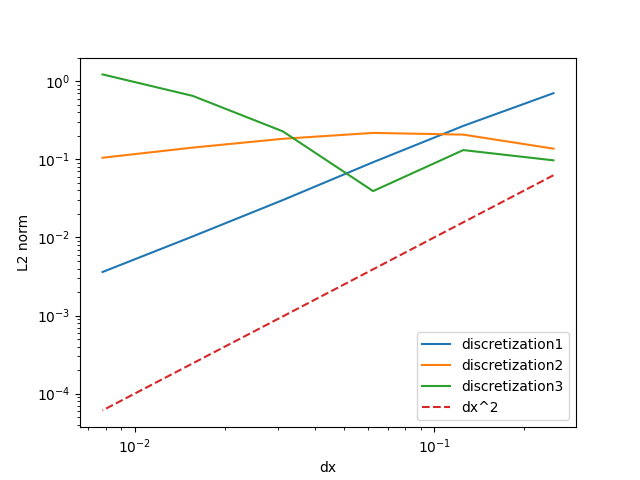
\includegraphics[width=0.45\textwidth]{task2_L2norm.png}
    \caption{Convergence plot of the $L^2$ norm of the error}
    \label{fig:L2norm}
\end{figure}

The results show different convergence behaviors for the three methods. 
The second-order central differencing scheme (Discretization1) shows a trend of second-order accuracy. This can be seen by the fact that the slope of the $L^2$ norm
follows the one of $\Delta x^2$ in the log-log plot. This behavior aligns with the theoretical expectation.

In contrast, the first-order upwind differencing method (Discretization 2) shows a much slower convergence: the error remains nearly constant for smaller $\Delta x$ values.
This result may suggest that numerical diffusion dominates the solution, and further grid refinement does not improve accuracy.
First-order schemes like upwind differencing are stable but suffer from significant numerical dissipation, especially for advection-dominated problems or at high Peclet numbers.

The second-order upwind method (Discretization 3) displays improved accuracy compared to the first-order upwind method, with the error reducing more significantly as  $\Delta x$ decreases.
However, the convergence behavior is less smooth, with some variability observed at intermediate grid sizes. This may result from the interplay between truncation errors and the Peclet number, which affects the balance between advection and diffusion.

\subsection{Comparison for different Peclet numbers}
To further investigate the impact of the Peclet number on the accuracy of the numerical solutions, we repeated the convergence analysis for different values of $Pe$, as indicated by the assignment.

\begin{figure}[h!]
    \centering
    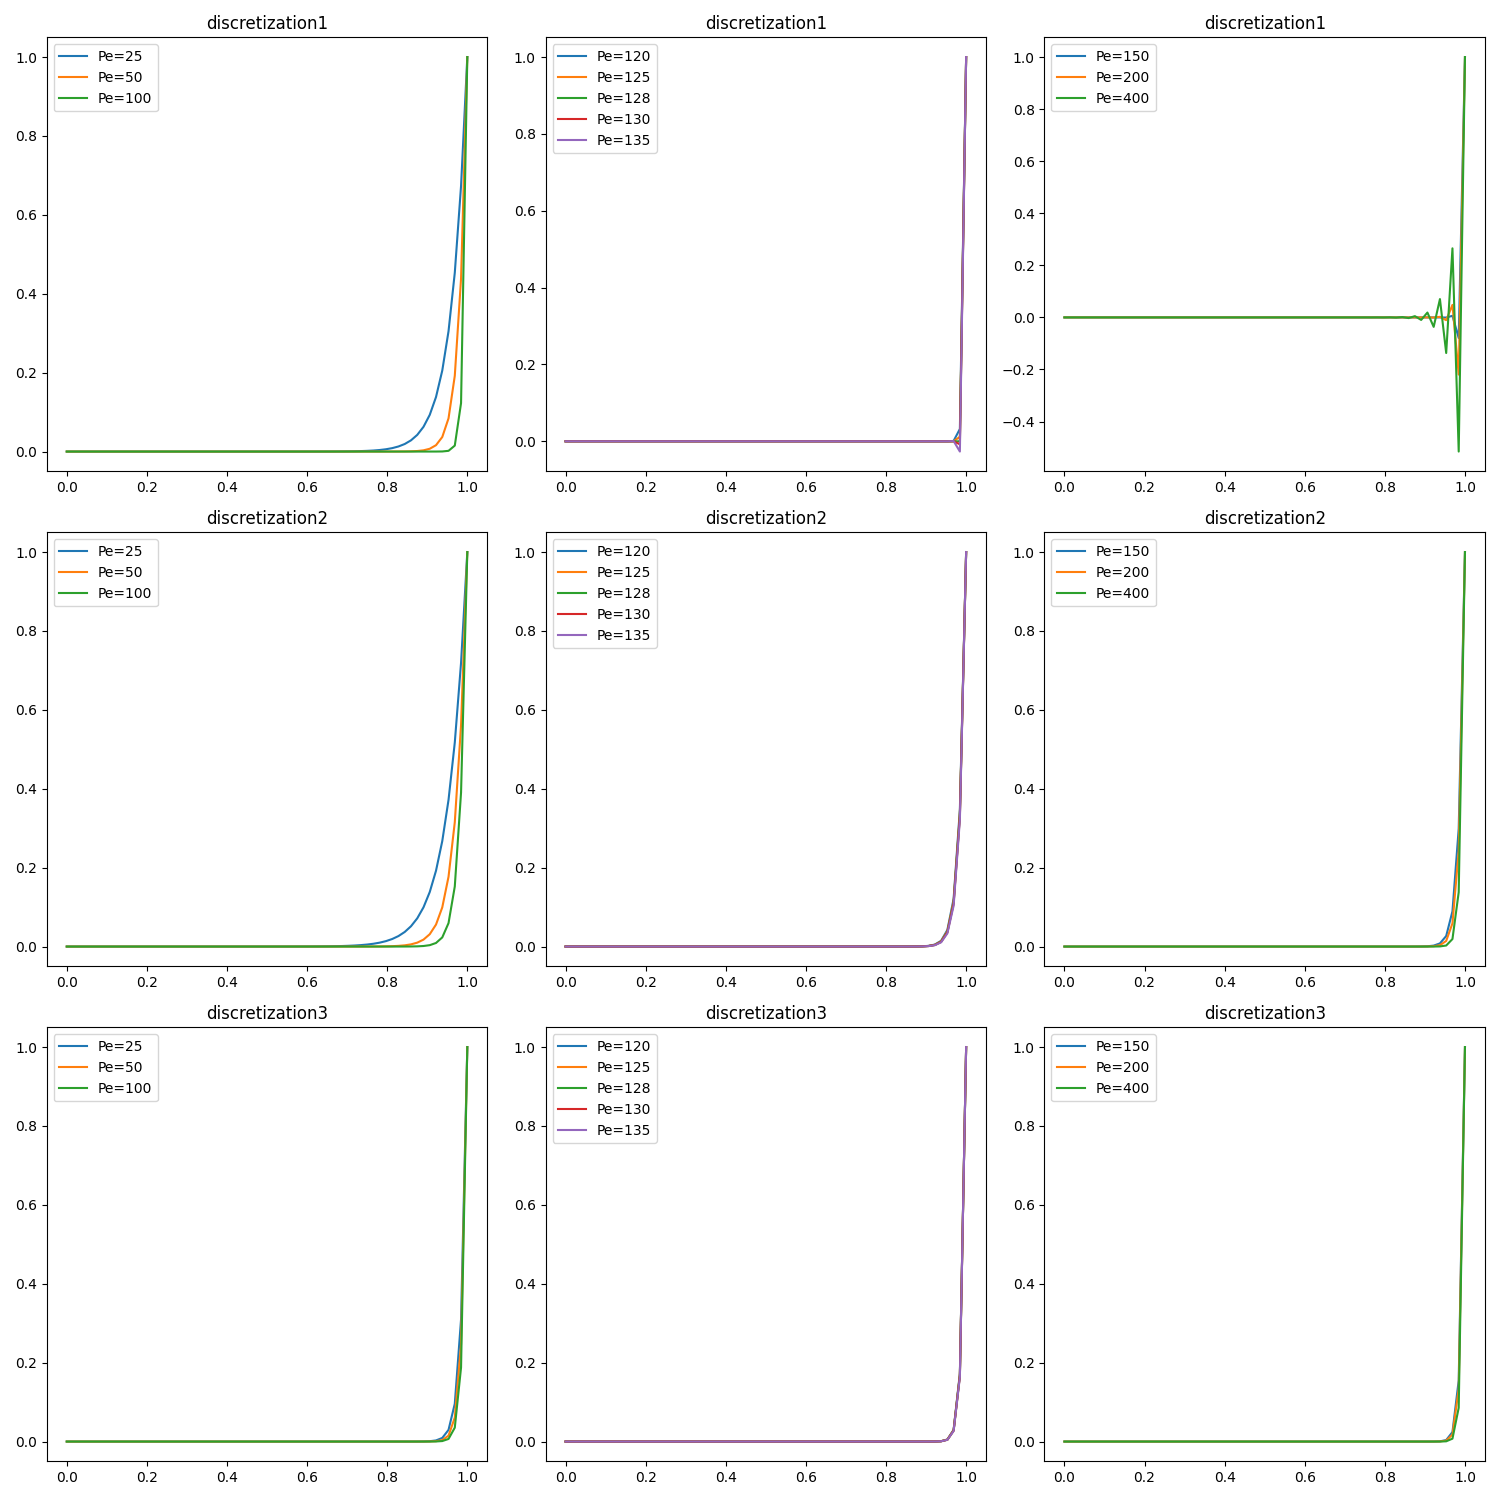
\includegraphics[width=0.45\textwidth]{task2_fixed_dx.png}
    \caption{Solutions for different Peclet numbers}
    \label{fig:L2norm_fixed_dx}
\end{figure}

From the picture above, we can observe that CDS discretization shows an oscillatory behavior for high Peclet numbers in particular for the region where the solution varies rapidly, while it provides high accuracy in regions where the solution varies smoothly.
This behavior may be due to the fact that the CDS is not a suitable method when the advection term is dominant, since it is not capturing the upwind information.

Focusing on the first-order upwind discretization, we can see that the solution is stable for all Peclet numbers, but for small Peclet values it is making the function smoother than it should be, because of the numerical dissipation.

In the end we can see that the second-order upwind discretization is able to capture the correct behavior of the solution, providing a good approximation and stability for all Peclet numbers.

All the three methods are described by sparse matrices, which reflects the local nature of the finite difference approximations, but the second-order upwind scheme, which provides the highest accuracy, requires more memory due to the larger stencil size.


\subsection{Comparison of the different methods}
For advection-dominated problems with medium to high Peclet numbers, the second-order upwind scheme is generally the best choice as it balances stability and accuracy effectively, avoiding any kind of oscillation.
For high Peclet values, we can also consider to use the first-order upwind scheme, since it is stable and does not show oscillations, it is also easier to implement and computationally cheaper than the second-order upwind scheme.
For problems in which we have a Peclet number close to 1 the CDS scheme is a viable option.



\section{Stability of the unsteady advection-diffusion equation}

\subsection{Discretization of of the unsteady one-dimensional advection-diffusion equation}


We start with the one-dimensional advection-diffusion equation:

\[
\rho \left( \frac{\partial \Phi}{\partial t} + U \frac{\partial \Phi}{\partial x} \right) = \alpha \frac{\partial^2 \Phi}{\partial x^2}.
\]

We use central finite differencing in space and explicit Euler in time. The terms are discretized as follows:

\begin{itemize}
    \item \(\frac{\partial \Phi}{\partial t} \approx \frac{\Phi_i^{n+1} - \Phi_i^n}{\Delta t}\)
    \item \(\frac{\partial \Phi}{\partial x} \approx \frac{\Phi_{i+1}^n - \Phi_{i-1}^n}{2\Delta x}\)
    \item \(\frac{\partial^2 \Phi}{\partial x^2} \approx \frac{\Phi_{i+1}^n - 2\Phi_i^n + \Phi_{i-1}^n}{\Delta x^2}\)
\end{itemize}

Substituting these approximations into the original equation, we get:

\[
\rho \left( \frac{\Phi_i^{n+1} - \Phi_i^n}{\Delta t} \right) + \rho U \left( \frac{\Phi_{i+1}^n - \Phi_{i-1}^n}{2\Delta x} \right) = \alpha \left( \frac{\Phi_{i+1}^n - 2\Phi_i^n + \Phi_{i-1}^n}{\Delta x^2} \right).
\]

Multiplying through by \(\Delta t\):

\[
\rho \Phi_i^{n+1} - \rho \Phi_i^n + \rho U \Delta t \left( \frac{\Phi_{i+1}^n - \Phi_{i-1}^n}{2\Delta x} \right) = \alpha \Delta t \left( \frac{\Phi_{i+1}^n - 2\Phi_i^n + \Phi_{i-1}^n}{\Delta x^2} \right).
\]

Rearranging to isolate \(\Phi_i^{n+1}\) on the left-hand side:

\[
\rho \Phi_i^{n+1} = \rho \Phi_i^n - \rho U \Delta t \left( \frac{\Phi_{i+1}^n - \Phi_{i-1}^n}{2\Delta x} \right) + \alpha \Delta t \left( \frac{\Phi_{i+1}^n - 2\Phi_i^n + \Phi_{i-1}^n}{\Delta x^2} \right).
\]

Dividing through by \(\rho\):

\begin{equation}
  \label{eq:discretized}
\Phi_i^{n+1} = \Phi_i^n - c \left( \frac{\Phi_{i+1}^n - \Phi_{i-1}^n}{2} \right) + d \left( \Phi_{i+1}^n - 2\Phi_i^n + \Phi_{i-1}^n \right),
\end{equation}

where:

\[
c = \frac{U \Delta t}{\Delta x}, \quad d = \frac{\alpha \Delta t}{\rho (\Delta x)^2}.
\]

The parameter $c$ represents the Courant number and quantifies the influence of advection in the simulation. 
For stability and accuracy in explicit schemes, $c$ should typically be small to satisfy the Courant-Friedrichs-Lewy condition that requires $c \leq 1$. 
If $c$ is too large, the simulation may become unstable or inaccurate because the flow travels across more than one grid cell per time step.
The parameter $d$ represents the Fourier number and measures the contribution of diffusion to the simulation.
The diffusion stability condition requires $d \leq 1/2$ to ensure that diffusion does not dominate excessively or destabilize the solution.


\subsection{Stability Analysis Using Von Neumann Method}
Given the discretized convection-diffusion equation \eqref{eq:discretized}, we can perform a Von Neumann stability analysis to determine the stability conditions for the explicit scheme. 
\\This is made possible due to the linear nature of such equation and by not considering the imact of boundary conditions. 
We will consider the domain as periodic in \(x\), allowing the solution and the error to be expressed using a Fourier series with a period of length \(2L\).

Assuming a disturbance of the form:

\[
\epsilon(x, t) = V(t) e^{ikx},
\]

where $\theta = k \Delta x$ is the phase angle.
\\We can insert the error function \(epsilon(x, t)\) into the discretized differential equation and estimate the temporal behaviour of the amplitude by evaluation the amplification factor \(G\). This can be directly applied to the solution, by exploiting the linearity of the equation so that:

\[
\phi_i^n = V^n e^{I \theta i}, \quad \phi_{i+1}^n = V^n e^{I \theta (i+1)}, \quad \phi_{i-1}^n = V^n e^{I \theta (i-1)}.
\]

Substituting into the discretized equation:

\[
V^{n+1} = V^n \left(1 - \frac{c}{2} (e^{I \theta} - e^{-I \theta}) + d (e^{I \theta} - 2 + e^{-I \theta})\right).
\]

By considering the Euler relation \(e^{I \theta} = \cos \theta + I \sin \theta\), we can simplify the equation to:

\[
V^{n+1} = V^n \left(1 - I c \sin \theta + 2d (\cos \theta - 1)\right).
\]

The amplification factor $G$, which can be computed for subsequent steps, is the following:

\[
G = 1 - i c \sin \theta + 2d (\cos \theta - 1).
\]

To obtain stability, by remembering that the amplification factor should damp the error to obtain stability, we require that the absolute value of $G$ is less than or equal to 1:

\[
|G| \leq 1.
\]

We then compute $|G|^2$ to find the stability condition on the real domain:

\[
|G|^2 = \left(1 + 2d (\cos \theta - 1)\right)^2 + (c \sin \theta)^2.
\]

For stability, we need to find the values of $c$ and $d$ that satisfy the condition:

\[
|G|^2 \leq 1.
\]

We can solve this with variable substitution and trigonometric identities to find the stability condition for the explicit scheme.
We get the following disequation:

\[
t^2(1-\frac{c^2}{4d^2}) + t(\frac{1}{d}-2) + 1 (1-\frac{1}{d}+\frac{c^2}{4d^2}) \leq 0.,
\]

where \(t = \cos \theta\).

We can thus solve it by applying the general quadratic formula to find the stability condition:

\begin{equation}
\frac{\frac{1}{d}-2-\sqrt{(\frac{1}{d}-2)^2-4(1-\frac{c^2}{4d^2})(1-\frac{1}{d}-\frac{c^2}{4d^2})}}{2(1-\frac{c^2}{4d^2})}\leq t
\end{equation}
\begin{equation}
t \leq \frac{\frac{1}{d}-2+\sqrt{(\frac{1}{d}-2)^2-4(1-\frac{c^2}{4d^2})(1-\frac{1}{d}-\frac{c^2}{4d^2})}}{2(1-\frac{c^2}{4d^2})}
\end{equation}

We can now substitute the values of \(c\) and \(d\) to find the stability condition for the explicit scheme.
We recall that \(c\)=\(\frac{U \Delta t}{\Delta x}\) and \(d\)=\(\frac{\alpha \Delta t}{\rho (\Delta x)^2}\).

By substituting this in the disequation we get:

\begin{equation}
\frac{\frac{\alpha \Delta t}{\rho (\Delta x)^2}-2-\sqrt{(\frac{\alpha \Delta t}{\rho (\Delta x)^2}-2)^2-4(1-\frac{U^2 \Delta t^2}{4 \alpha \Delta x^2})(1-\frac{\alpha \Delta t}{\rho (\Delta x)^2}-\frac{U^2 \Delta t^2}{4 \alpha \Delta x^2})}}{2(1-\frac{U^2 \Delta t^2}{4 \alpha \Delta x^2})}\leq t
\end{equation}
\begin{equation}
  t \leq \frac{\frac{\alpha \Delta t}{\rho (\Delta x)^2}-2+\sqrt{(\frac{\alpha \Delta t}{\rho (\Delta x)^2}-2)^2-4(1-\frac{U^2 \Delta t^2}{4 \alpha \Delta x^2})(1-\frac{\alpha \Delta t}{\rho (\Delta x)^2}-\frac{U^2 \Delta t^2}{4 \alpha \Delta x^2})}}{2(1-\frac{U^2 \Delta t^2}{4 \alpha \Delta x^2})}
\end{equation}
Given the complexity of the disequation, it is beneficial to analyze the two extreme cases: \(\theta = 0\) and \(\theta = \pi\).

\begin{enumerate}
  \item \textbf{Case 1: \( \theta = \pi \) (Maximum Frequency)}

  At \( \theta = \pi \), we have:

  \[
  \cos \pi = -1, \quad \sin \pi = 0.
  \]

  Substitute into the expression for \( G \):

  \[
  G = 1 + 2d (-1 - 1) = 1 - 4d.
  \]

  The magnitude is:

  \[
  |G|^2 = (1 - 4d)^2.
  \]

  For instability, we need:

  \[
  (1 - 4d)^2 > 1.
  \]

  Taking the square root:

  \[
  |1 - 4d| > 1.
  \]

  This gives two conditions:

  \[
  1 - 4d > 1 \quad \text{or} \quad 1 - 4d < -1.
  \]

  Solving these inequalities:

  \begin{enumerate}
    \item \( 1 - 4d > 1 \implies d < 0 \) (not physically meaningful),
    \item \( 1 - 4d < -1 \implies d > \frac{1}{2} \).
  \end{enumerate}

  Thus, \textbf{instability occurs at \( \theta = \pi \) when \( d > \frac{1}{2} \)}.
  Substituting \( d = \frac{\alpha \Delta t}{\rho (\Delta x)^2} \) into the instability condition \( d > \frac{1}{2} \):

  \[
  \frac{\alpha \Delta t}{\rho (\Delta x)^2} > \frac{1}{2}.
  \]

  Rearranging to find the relationship between \( \Delta x \) and \( \Delta t \):

  \[
  \Delta t < \frac{\rho (\Delta x)^2}{2 \alpha}.
  \]

  This inequality provides the stability condition for the explicit scheme in terms of the time step \( \Delta t \) and the spatial step \( \Delta x \). For the scheme to be stable, the time step must be sufficiently small relative to the square of the spatial step.

  \item \textbf{Case 2: \( \theta \approx 0 \) (Low Frequencies)}

  For small \( \theta \), we use the Taylor expansions:

  \[
  \sin \theta \approx \theta, \quad \cos \theta \approx 1 - \frac{\theta^2}{2}.
  \]

  Substitute into the expression for \( G \):

  \[
  G \approx 1 - d \theta^2 - i c \theta.
  \]

  Compute \( |G|^2 \):

  \[
  |G|^2 \approx (1 - d \theta^2)^2 + (c \theta)^2.
  \]

  Neglecting terms of order \( \theta^4 \), we get:

  \[
  |G|^2 \approx 1 - 2d \theta^2 + c^2 \theta^2.
  \]

  For instability, we need:

  \[
  1 - 2d \theta^2 + c^2 \theta^2 > 1.
  \]

  Canceling the 1:

  \[
  -2d \theta^2 + c^2 \theta^2 > 0,
  \]

  or:

  \[
  (c^2 - 2d) \theta^2 > 0.
  \]

  For instability, this implies:

  \[
  c^2 > 2d.
  \]
  Substituting \( c = \frac{U \Delta t}{\Delta x} \) and \( d = \frac{\alpha \Delta t}{\rho (\Delta x)^2} \) into the instability condition \( c^2 > 2d \):

  \[
  \left( \frac{U \Delta t}{\Delta x} \right)^2 > 2 \left( \frac{\alpha \Delta t}{\rho (\Delta x)^2} \right).
  \]

  Simplifying:

  \[
  \frac{U^2 (\Delta t)^2}{(\Delta x)^2} > \frac{2 \alpha \Delta t}{\rho (\Delta x)^2}.
  \]

  Multiplying both sides by \( (\Delta x)^2 \):

  \[
  U^2 (\Delta t)^2 > \frac{2 \alpha \Delta t}{\rho}.
  \]

  Dividing both sides by \( \Delta t \):

  \[
  U^2 \Delta t > \frac{2 \alpha}{\rho}.
  \]

  Rearranging to find the relationship between \( \Delta x \) and \( \Delta t \):

  \[
  \Delta t < \frac{2 \alpha}{\rho U^2}.
  \]

  Thus, the stability condition for the explicit scheme, considering both advection and diffusion, is:

  \[
  \Delta t < \min \left( \frac{\rho (\Delta x)^2}{2 \alpha}, \frac{2 \alpha}{\rho U^2} \right).
  \]
\end{enumerate}

\subsection{Stability region}
\begin{figure}[h]
  \centering
  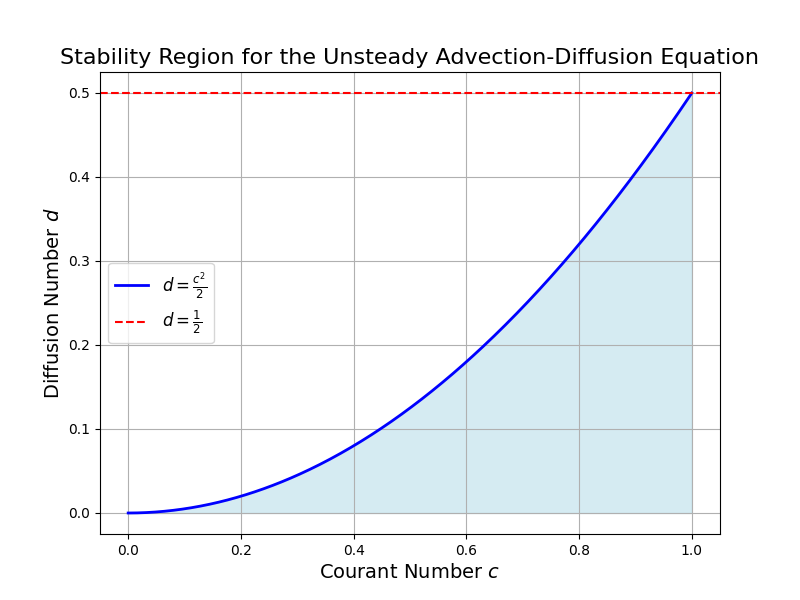
\includegraphics[width=0.8\textwidth]{stability_region_plot.png}
  \caption{Stability region for the explicit scheme.}
  \label{fig:stability_region}
\end{figure}


\section{Numerical solution of the unsteady advection-diffusion equation}

The attached file \texttt{task4.py} from our repository \cite{GitHubRepo} contains the Python code which should be executed to obtain 
the numerical solution of the unsteady advection-diffusion equation using different discretization methods respectively: second-order central 
differencing, first- and second-order upwind differencing.The solutions are included in this report, as requested. In the case of an explicit 
scheme, the solution obtained using the Central Difference Scheme is stable only for low Peclet numbers, as the diffusion phenomenon dominates 
over advection. For higher Peclet numbers, the solution becomes unconditionally unstable due to the dominance of the advection term.
On the contrary, using the first- and second-order upwind methods, the largest allowed time-step based on coefficient analysis is:

\[
\Delta t < \min \left( \frac{\rho (\Delta x)^2}{2 \alpha}, \frac{\Delta x}{U} \right),
\]



\begin{figure}[h!]
  \centering
  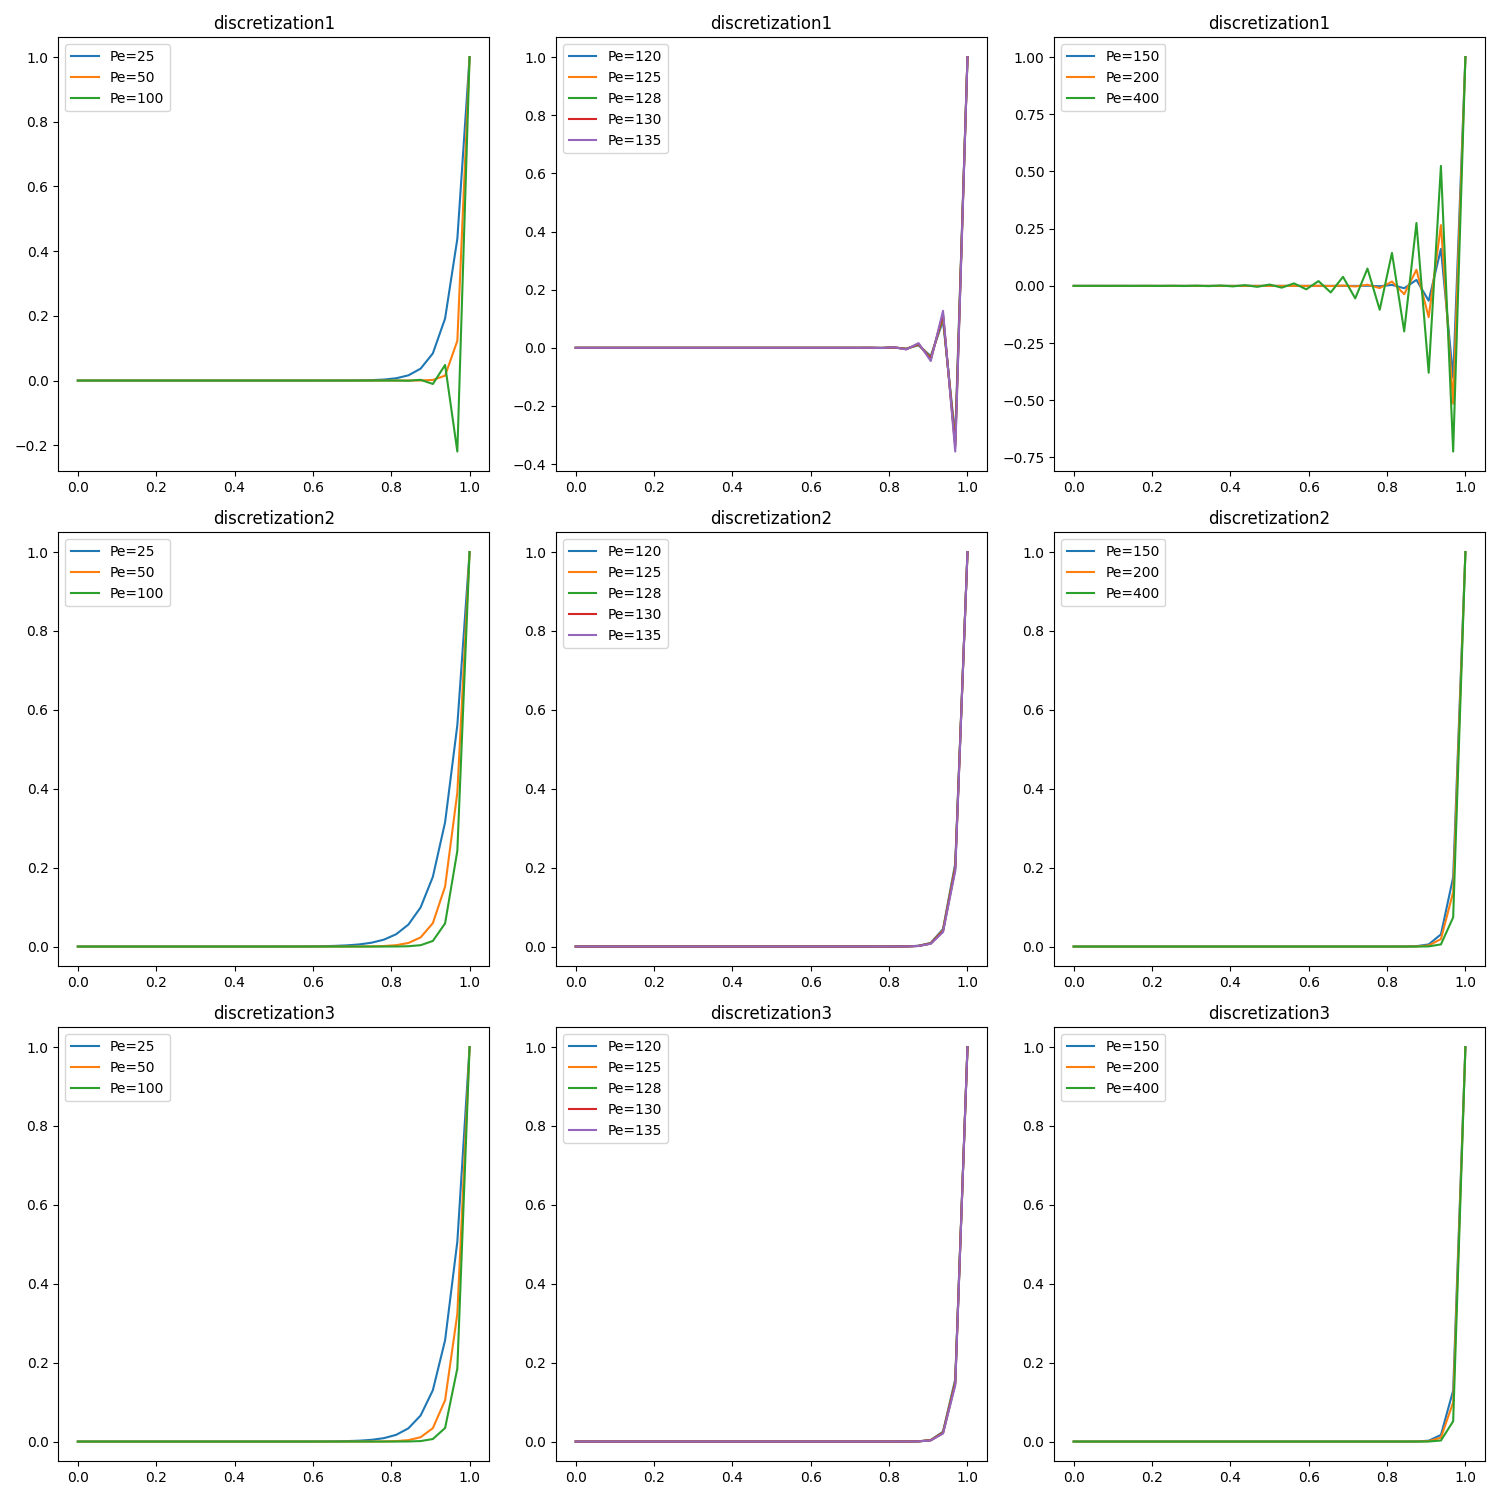
\includegraphics[width=0.5\textwidth]{task4.png}
  \caption{Numerical solution of the unsteady advection-diffusion equation}
  \label{fig:Numerical solution of the unsteady advection-diffusion equation}
\end{figure}


\section{Wave speed and minimum required grid resolution}

\subsection{Connection between grid resolution and the wave number of the ine wave}

To accurately represent a sine wave on a grid, the grid resolution $\Delta x$ must be such that there are at least 2 grid points per wavelength.
The smallest allowable wavelenght is:

\[
\lambda_{\text{min}} = 2 \Delta x
\]
Since the wavelength $\lambda$ and the wavenumber $k$ are related, the maximal wave number $k_{\text{max}}$ that can be resolved by the grid is:

\[
\lambda = \frac{2\pi}{k} \implies k_{\text{max}} = \frac{\pi}{\Delta x}
\]
If \( k > k_{\text{max}} \), the sine wave cannot be correctly represented. In particular, for coarser grids $\frac{\Delta x}{16}$ the 
high-wavenumber waves \( k = 8, 16 \) exhibit numerical dissipation and the sine wave appear damped due to insufficient resolution. For finer
grids all of the sine wave are well within the limit and should be resolved correctly. However, as k increases, the accuracy may decrease slightly
due to numerical errors.

\subsection{Ideal behavior for each Pe}

For \( Pe = 25 \) the ideal behavior is a damped sine wave over time because the diffusion term introduces energy dissipation, reducing the
wave amplitude. Higher wavenumbers k are affected more because diffusion acts more strongly on smaller wavelengths. Thus, diffusion plays a 
significant role. For \( Pe \to \infty \) diffusion is negligible and he ideal behavior is a pure advection of the sine wave, meaning the wave 
travels at a constant speed without any change in amplitude or shape.

\subsection{Turbulent flow}
A turbulent flow can be thought of as the combination of different waves with different wavenumbers. To accurately simulate turbulent flows, 
the numerical scheme should minimize diffusion that distort the wave amplitude and phase. 

Central Difference Scheme provides second-order accuracy and does well for lower wavenumbers but is is prone to numerical dispersion errors, 
especially at high wavenumbers and high Peclet numbers so It may generate oscillations or instabilities when the grid resolution is not sufficient.

First-Order Upwind Scheme is inherently stable and free from oscillations, even at high Peclet numbers. However, introduces numerical diffusion 
which causes significant damping of high-wavenumber waves so is not ideal for turbulent flows because its numerical diffusion suppresses high-frequency components.

Second-Order Upwind Scheme is more accurate and better at preserving wave amplitudes at higher Peclet numbers leading to better representation of high-wavenumber waves, 
so it is a better choice for simulating a turbulent flow because it provides a balance between numerical stability and resolution of high-wavenumber components.

\begin{figure}[h!]
    \centering
    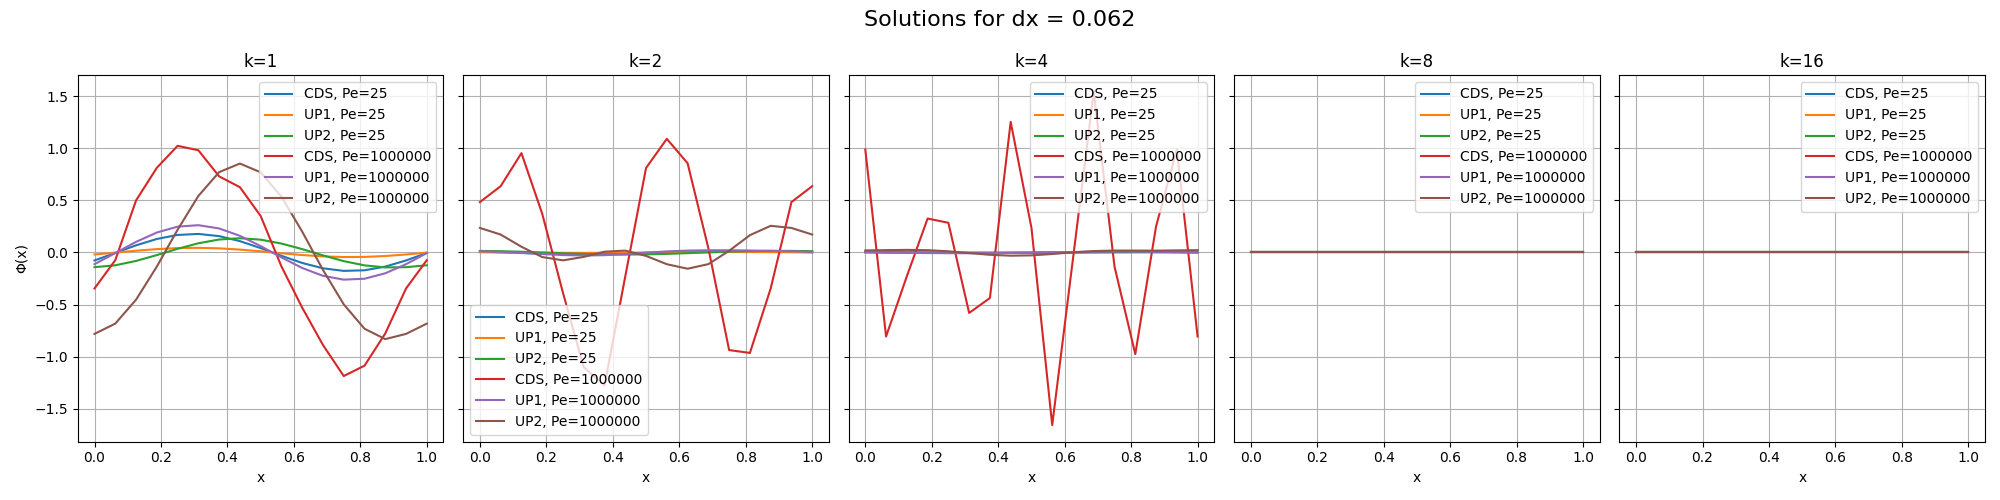
\includegraphics[width=1\textwidth]{task5_dx_16.png}
    \caption{Periodic boundary condition for \(\frac{\Delta x}{16}\).}
    \label{fig:periodic_dx_16}
\end{figure}

\begin{figure}[h!]
    \centering
    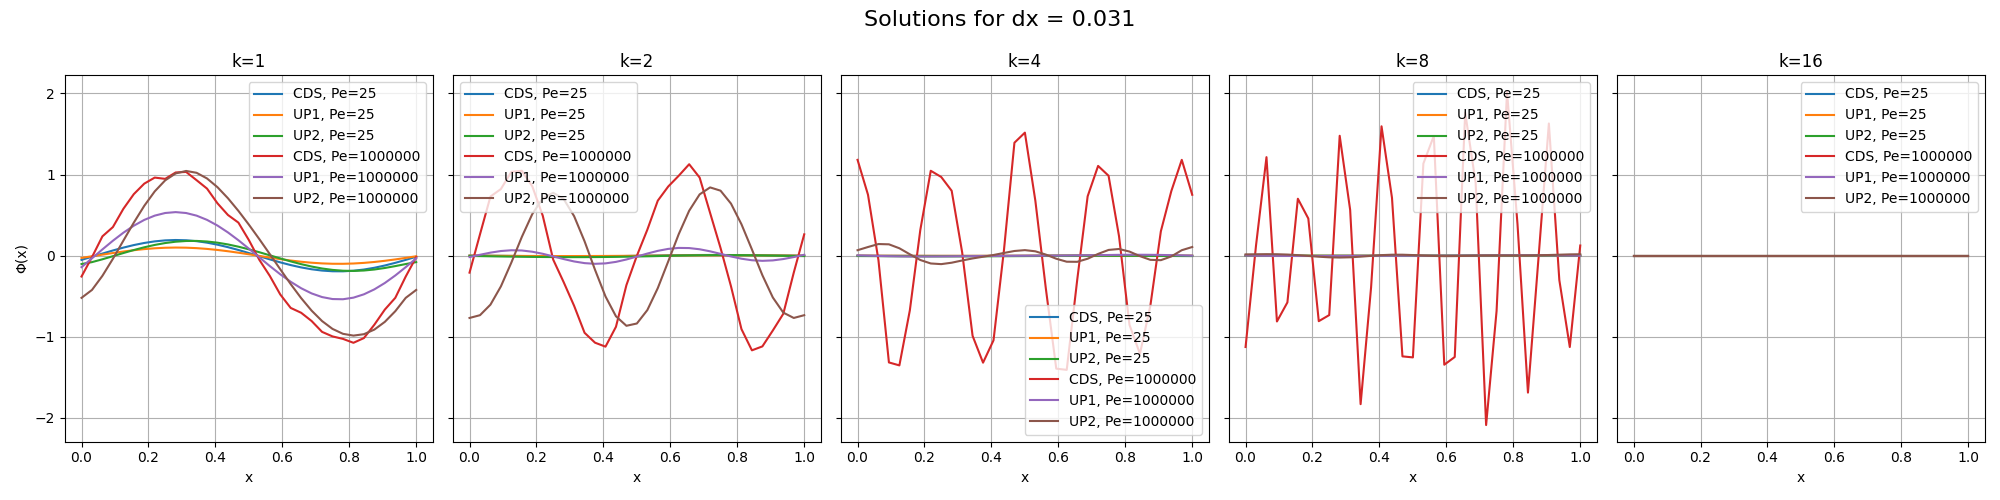
\includegraphics[width=1\textwidth]{task5_dx_32.png}
    \caption{Periodic boundary condition for \(\frac{\Delta x}{32}\).}
    \label{fig:periodic_dx_32}
\end{figure}

\begin{figure}[h!]
    \centering
    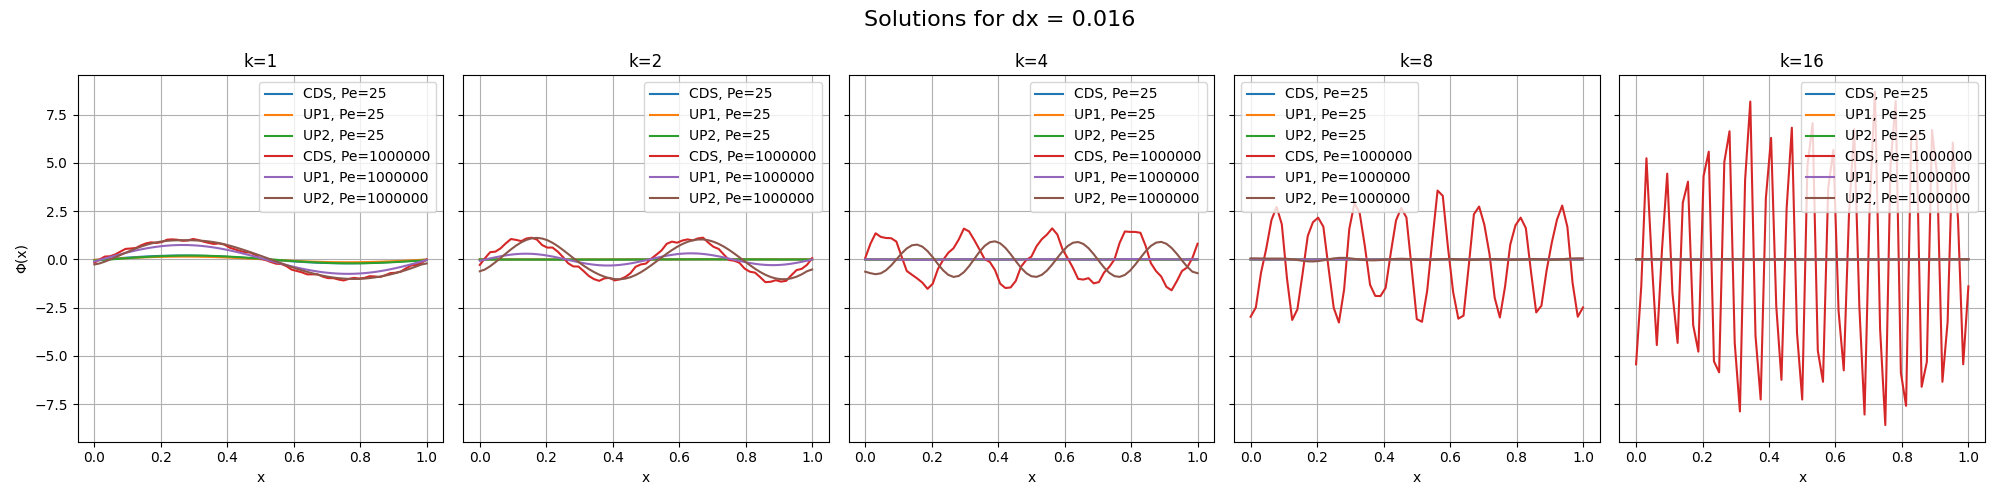
\includegraphics[width=1\textwidth]{task5_dx_64.png}
    \caption{Periodic boundary condition for \(\frac{\Delta x}{64}\).}
    \label{fig:periodic_dx_64}
\end{figure}

\begin{thebibliography}{9}
  \bibitem{GitHubRepo}
  \textit{CFD Repository},\\
  Available at: \url{https://github.com/GiuseppePisante/CFD.git}
  
  \bibitem{GitHubCopilot}
  \textit{GitHub Copilot},\\
  GitHub. Available at: \url{https://github.com/features/copilot}

\end{thebibliography}
\end{document}